\documentclass{beamer}
%% Possible paper sizes: a0, a0b, a1, a2, a3, a4.
%% Possible orientations: portrait, landscape
%% Font sizes can be changed using the scale option.
\usepackage[size=a3,orientation=landscape,scale=1.8]{beamerposter}
\usetheme{LLT-poster}
\usecolortheme{ComingClean}
% \usecolortheme{Entrepreneur}
% \usecolortheme{ConspiciousCreep}  %% VERY garish.

\usepackage[utf8]{inputenc}
\usepackage[T1]{fontenc}
\usepackage{libertine}
\usepackage[scaled=0.92]{inconsolata}
\usepackage[libertine]{newtxmath}

\usepackage{mwe}

\author[liantze@gmail.com]{Lim Lian Tze}
\title{Yet Another beamerposter Theme\\(Variable Sizes and Colour Themes)}
\institute{Your Institution}
% Optional foot image
\footimage{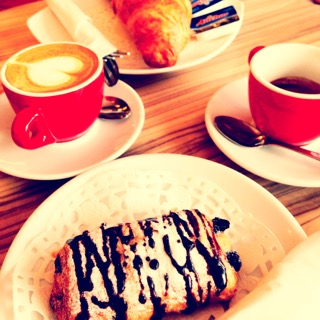
\includegraphics[width=4cm]{IMG_1934.jpg}}

\begin{document}
\begin{frame}[fragile]
\begin{columns}[T]

%%%% First Column
\begin{column}{.33\textwidth}

\begin{block}{Overview}
\begin{itemize}
\item This is the template I created for my poster presentations.
\item You can provide an optional \verb|\footimage|.
\end{itemize}
\end{block}

\begin{block}{Options}
\begin{itemize}
\item It's based on \texttt{beamerposter}, so you can change some options:
  \begin{description}
  \item[size] a0, a0b, a1, a2, a3, a4
  \item[orientiation] landscape, portrait
  \item[scale] a decimal number to scale the fonts
  \end{description}
\end{itemize}
\end{block}

\begin{block}{Colour Themes}
\begin{itemize}
\item I've included some colour themes, using the colour palettes from \url{http://colourlovers.com}
\begin{itemize}
\item ComingClean (teak and cream)
\item Entrepreneur (current theme)
\item Conspicious (a bit garish!)
\end{itemize}
\end{itemize}
\end{block}

\end{column}

%%%% Second Column
\begin{column}{.3\textwidth}

\begin{block}{This is a sample}
\begin{itemize}
\item One, two, pick up my shoe
\item Three, four, shut the door
\item Five, six, pick up sticks
\item Seven, eight, lay them straight
\item Nine, ten, a big fat hen
\item One, two, pick up my shoe
\item Three, four, shut the door
\item Five, six, pick up sticks
\item Seven, eight, lay them straight
\item Nine, ten, a big fat hen
\end{itemize}
\end{block}


\begin{block}{This is another sample}
\begin{itemize}
\item Some maths material
\begin{align}
A &= U \times S \times V^T\\
\sigma &= \frac{x\times y}{\sqrt[3]{\alpha + \beta}}
\end{align}
\end{itemize}
\end{block}
\end{column}

%%%% This is the THIRD column
\begin{column}{.33\textwidth}
\begin{block}{Brighten it up!}
This particular colour theme could do with some colourful images to brighten it up -- go wild with your charts!

\begin{center}
\includegraphics[width=.6\linewidth]{example-grid-100x100bp}
\end{center}

\end{block}
\end{column}

\end{columns}

\begin{block}{This is a sample of a wiiiide column}
\begin{itemize}
\item One, two, pick up my shoe
\item Three, four, shut the door
\item Five, six, pick up sticks
\item Seven, eight, lay them straight
\item Nine, ten, a big fat hen
\end{itemize}
\end{block}


\end{frame}
\end{document}